%%%% fatec-article.tex, 2024/03/10

\documentclass[
  a4paper,%% Tamanho de papel: a4paper, letterpaper (^), etc.
  12pt,%% Tamanho de fonte: 10pt (^), 11pt, 12pt, etc.
  english,%% Idioma secundário (penúltimo) (>)
  brazilian,%% Idioma primário (último) (>)
]{article}

%% Pacotes utilizados
\usepackage[]{fatec-article}

%% Início do documento
\begin{document}
\vspace{8cm}
\begin{center}
    \large \textbf{\title{ARTEFATOS DO PROJETO DE SOFTWARE}}
\end{center}

\maketitle

\break

\tableofcontents

\break


%exemplo da forma de organização das seções e subseções, você deverá adaptar o template para a realidade do seu projeto.

\section*{Diagramas}
Nesta seção serão apresentados os diagramas utilizados para a modelagem do sistema desenvolvido. Dentre os diagramas utilizados, podemos citar: Diagrama de Caso de Uso, Diagrama de Infraestrutura de Rede e os Modelos de Banco de Dados.
    
\subsection*{Diagrama de Caso de Uso}
\addcontentsline{toc}{section}{Diagrama de Caso de Uso}

    Nosso diagrama de casos de uso mostra como cada usuário pode interagir com o app para: abrir chamados, ver seu histórico de chamados e mudar o tipo de usuário que ele representa (se é um freelancer ou um cliente).

\begin{figure}[h]
\centering
\caption{Diagrama de caso de uso}%
\label{fig:diagrama-caso-uso}
 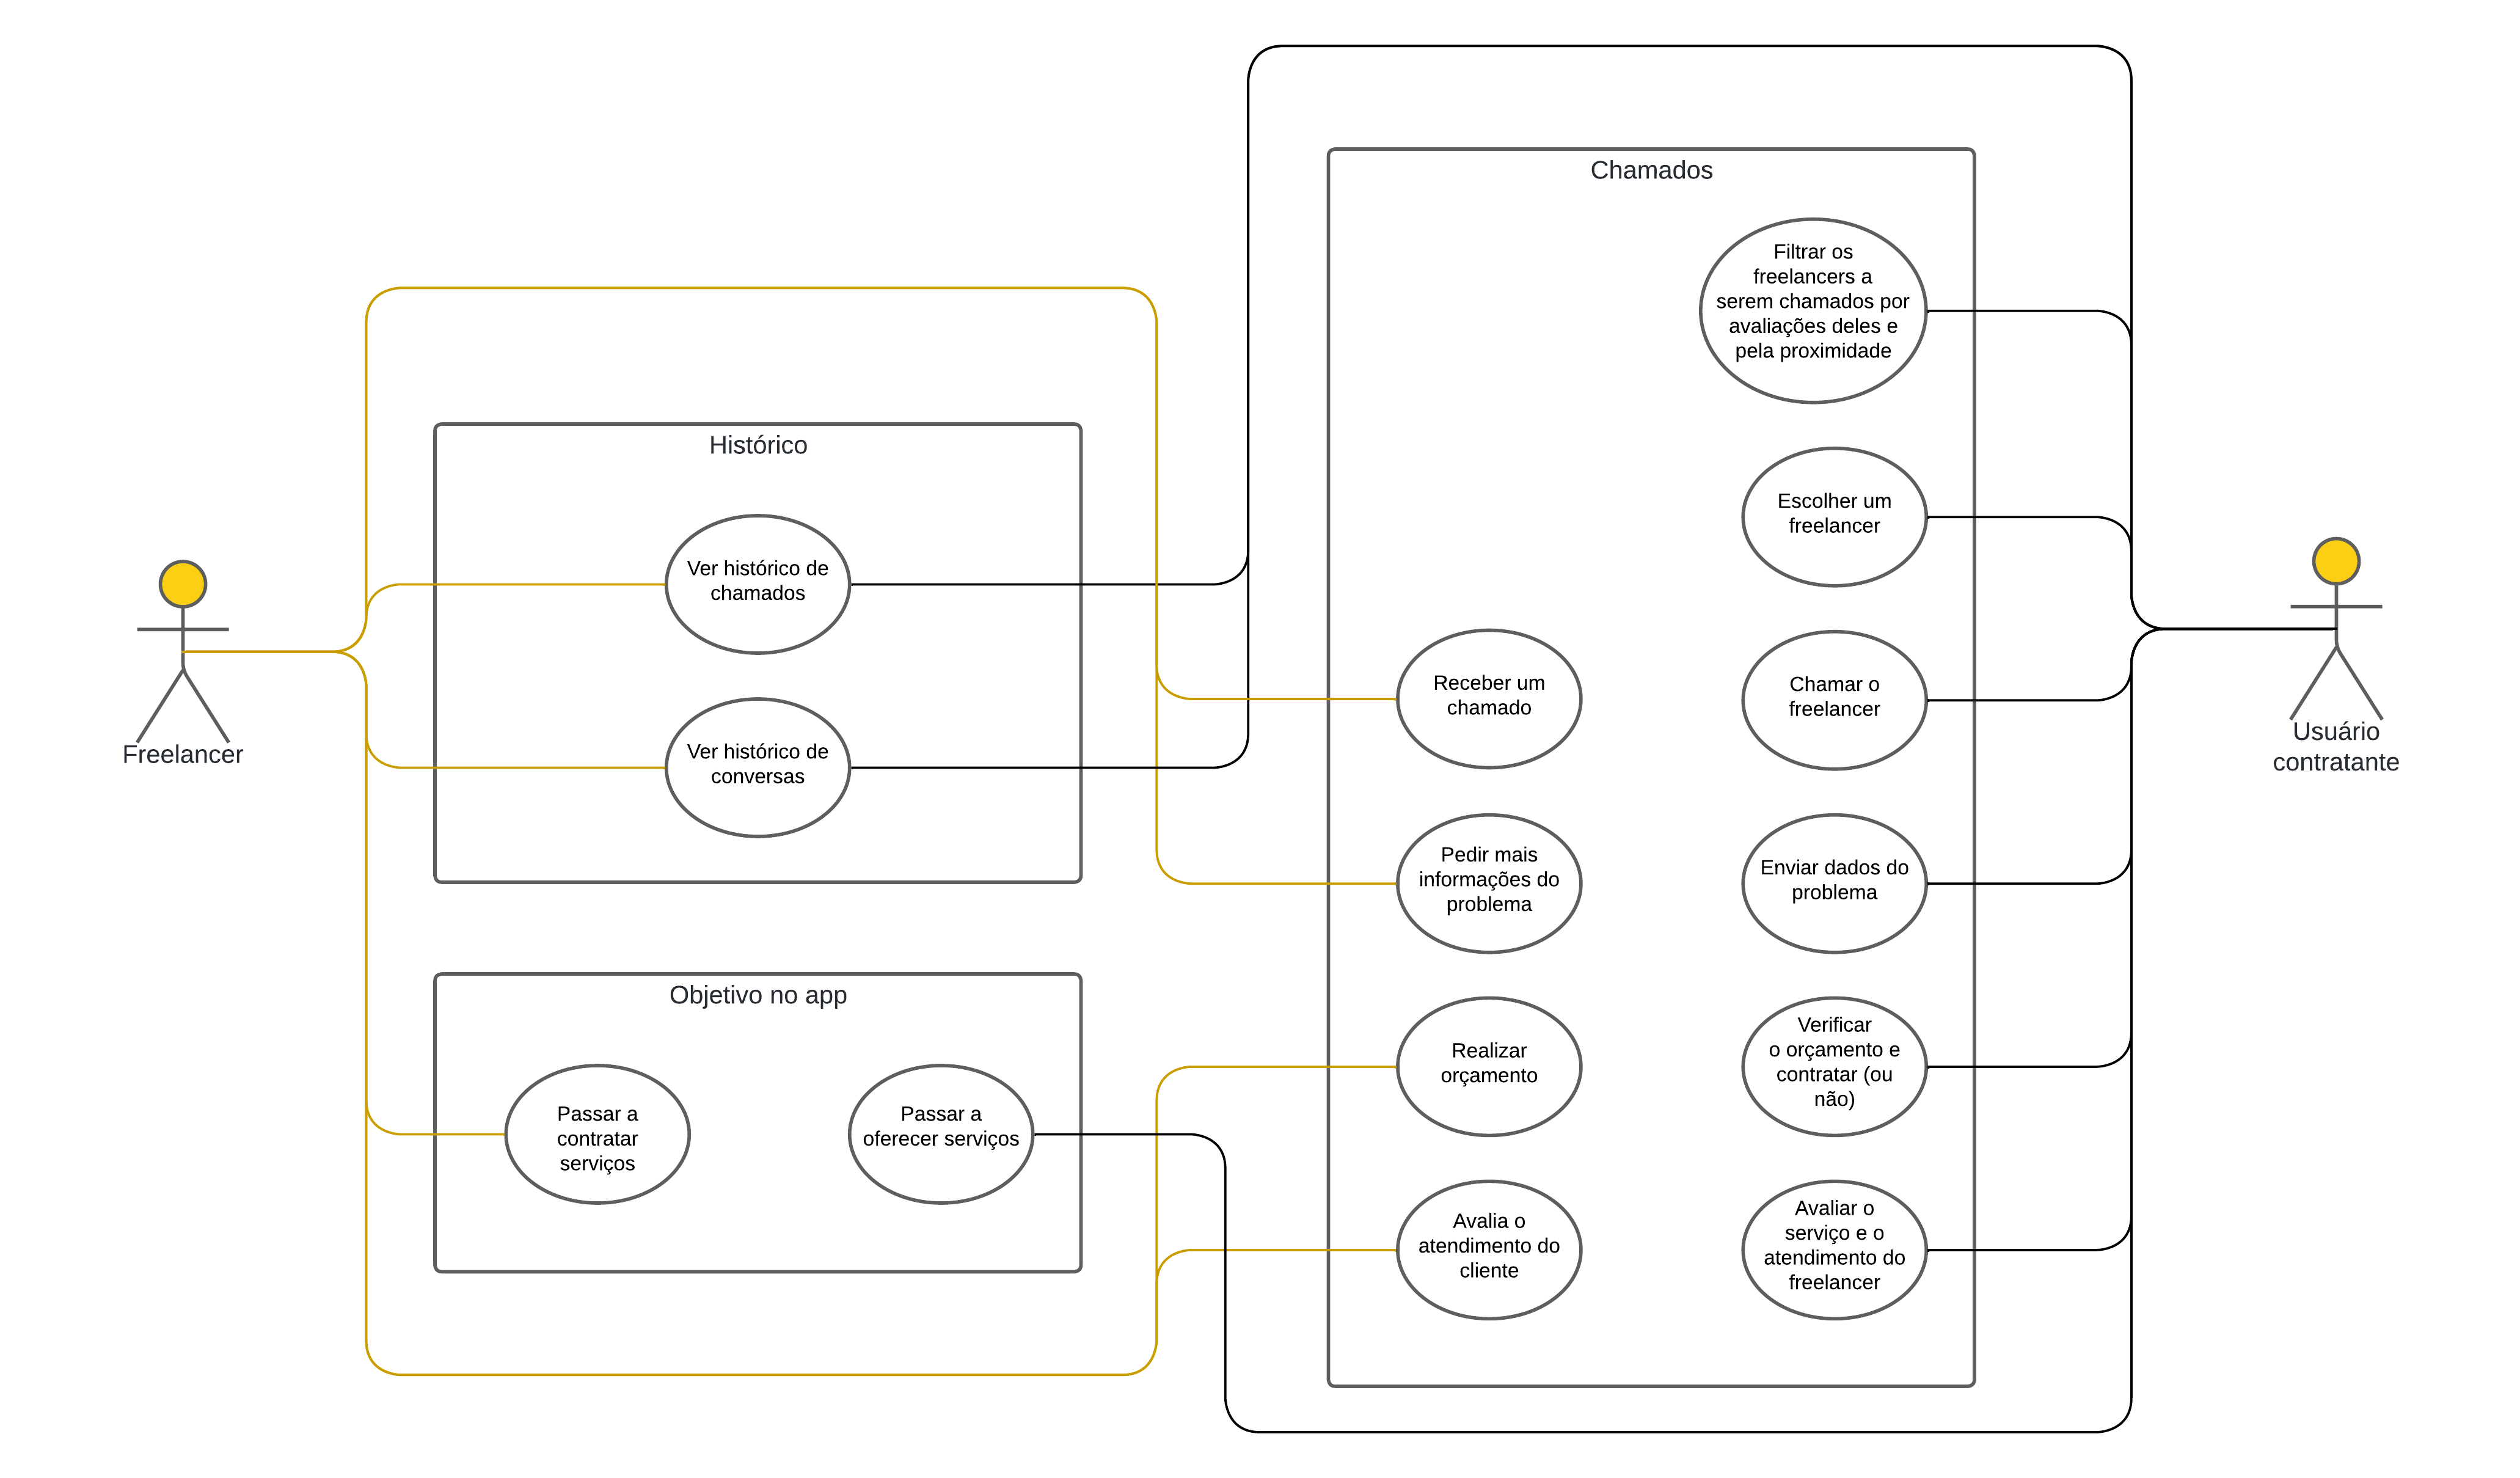
\includegraphics[width=1.1\textwidth]{fotos/casos de uso.png}
\SourceOrNote{Autoria própria (2024)}
\end{figure}

    As linhas amarelas saem do usuário freelancer, indo até cada ação que ele pode fazer e as linhas pretar indicam as ações dos usuários clientes

\break

\subsection*{Diagrama de Classes}
\addcontentsline{toc}{section}{Diagrama de Classes}

    Nosso diagrama de casos de uso mostra como cada usuário pode interagir com o app para: abrir chamados, ver seu histórico de chamados e mudar o tipo de usuário que ele representa (se é um freelancer ou um cliente).

\begin{figure}[h]
\centering
\caption{Diagrama de Classes}%
\label{fig:diagrama-classe}
 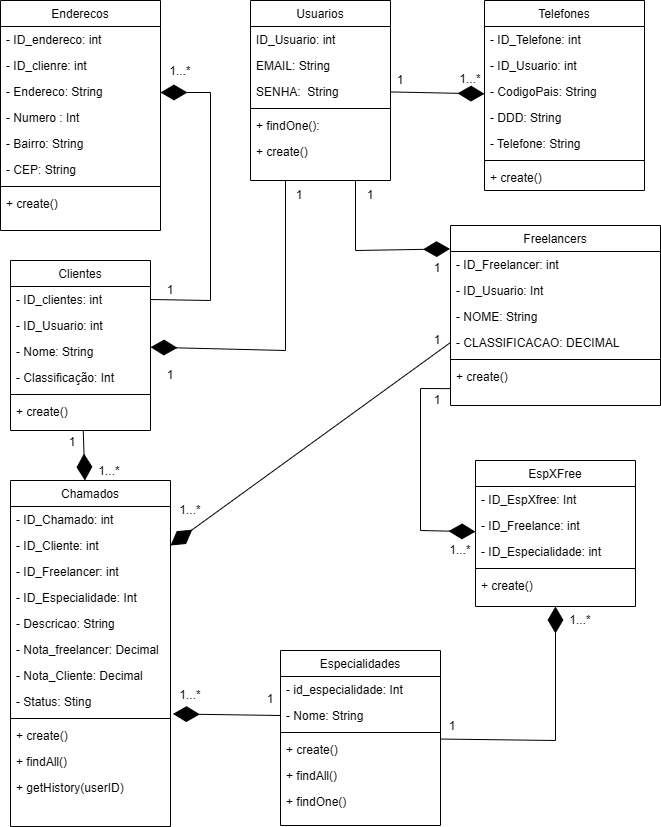
\includegraphics[width=0.8\textwidth]{fotos/diagramaClassePI.png}
\SourceOrNote{Autoria própria (2024)}
\end{figure}

    As linhas amarelas saem do usuário freelancer, indo até cada ação que ele pode fazer e as linhas pretar indicam as ações dos usuários clientes

\break

\subsection*{Diagrama de Objetos}
\addcontentsline{toc}{section}{Diagrama de Objetos}

    Nosso diagrama de casos de uso mostra como cada usuário pode interagir com o app para: abrir chamados, ver seu histórico de chamados e mudar o tipo de usuário que ele representa (se é um freelancer ou um cliente).

\begin{figure}[h]
\centering
\caption{Diagrama de objetos}%
\label{fig:diagrama-objetos}
 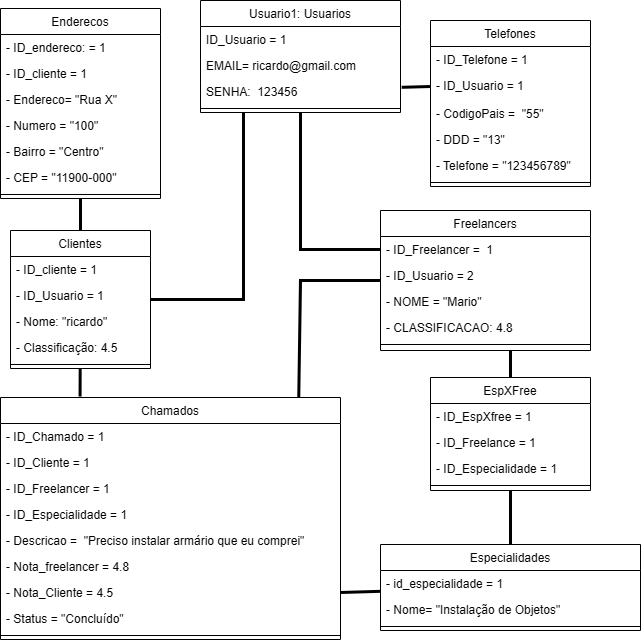
\includegraphics[width=0.8\textwidth]{fotos/DiagramaObjetopi.png}
\SourceOrNote{Autoria própria (2024)}
\end{figure}

    As linhas amarelas saem do usuário freelancer, indo até cada ação que ele pode fazer e as linhas pretar indicam as ações dos usuários clientes

\break
    
\subsection*{Diagrama de Infraestrutura de Rede}
\addcontentsline{toc}{section}{Diagrama de Infraestrutura de Rede}

    Esse diagrama mostra como o aplicativo seria hospedado, como chegaria aos usuários e como seria um possível escritório da empresa, mostrando as conexôes das redes.

\begin{figure}[h]
\centering
\caption{Diagrama de Infraestrutura de Rede}%
\label{fig:diagrama-classe}
 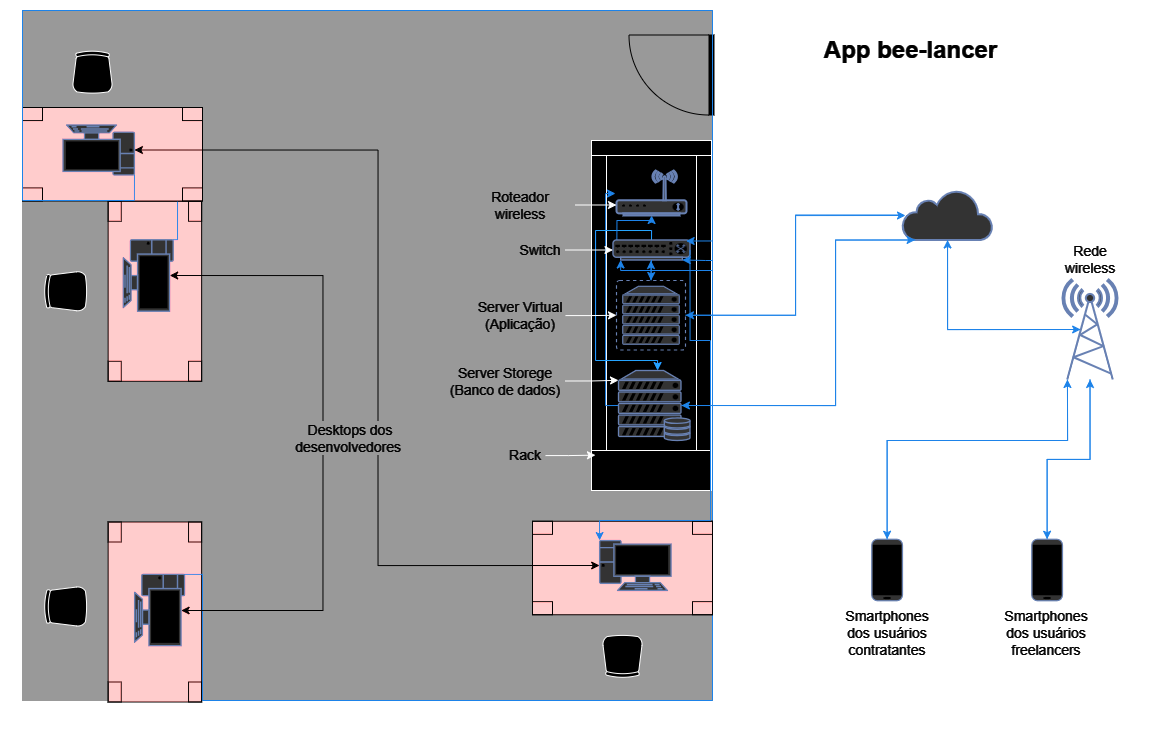
\includegraphics[width=1\textwidth]{fotos/Diagrama de Infraestrutura de Rede PI.png}
\SourceOrNote{Autoria própria (2024)}
\end{figure}

     As linhas azuis representam conexões da rede que podem ser feitas por cabos ou não.

\break

\subsection*{Modelo conceitual de Banco de dados}
\addcontentsline{toc}{section}{Modelo Conceitual de Banco de Dados}

    O modelo conceitual feito no BrModelo mostra todas as entidades, atributos, relacionamentos e cardinalidades necessárias para o seu entendimento e criação do banco de dados físico.

\begin{figure}[h]
\centering
\caption{Modelo Conceitual de Banco de Dados}%
\label{fig:diagrama-objetos}
 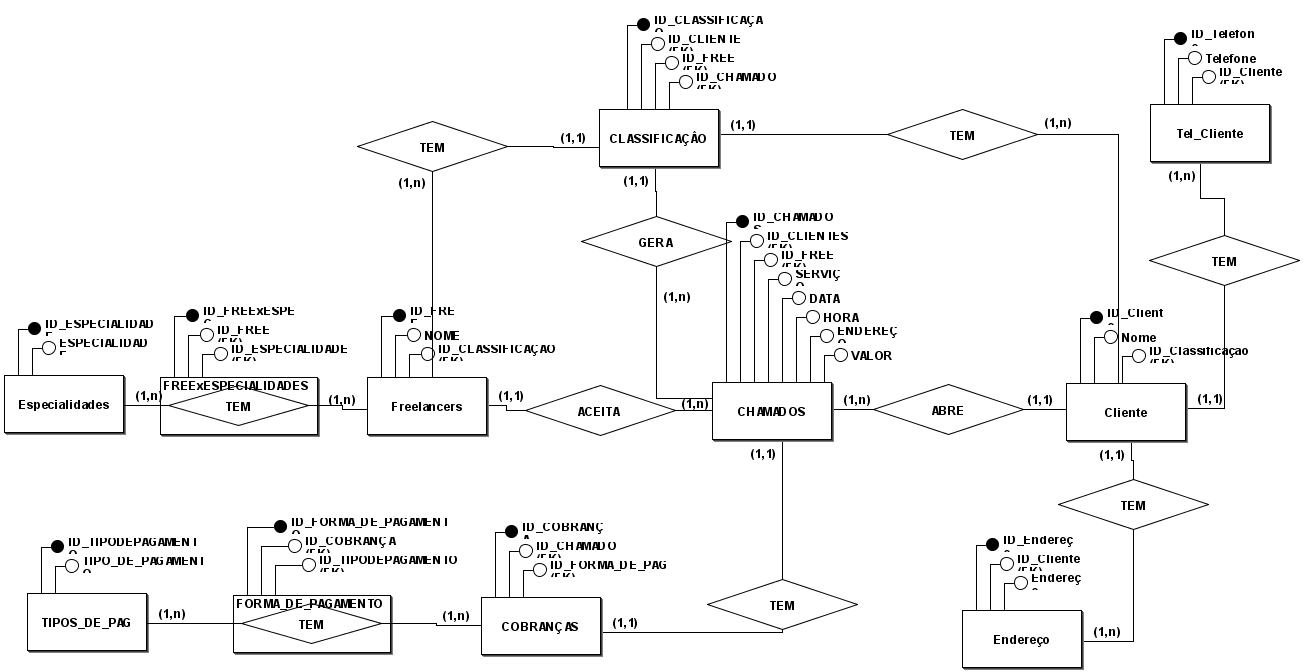
\includegraphics[width=1\textwidth]{fotos/modelo conceitual banco de dados.png}
\SourceOrNote{Autoria própria (2024)}
\end{figure}

    O seu formato mostra o máximo de detalhamento do banco de dados para facilitar no seu entendimento.

\break

\subsection*{Modelo lógico de Banco de dados}
\addcontentsline{toc}{section}{Modelo Lógico de Banco de Dados}

    O modelo lógico feito no BrModelo mostra todas as entidades, atributos, relacionamentos e cardinalidades no formato de tabelas interligadas para facilitar principalmente na criação do banco de dados físico.

\begin{figure}[h]
\centering
\caption{Modelo Lógico de Banco de Dados}%
\label{fig:diagrama-objetos}
 \includegraphics[width=1\textwidth]{fotos/Modelo lógico banco de dados.png}
\SourceOrNote{Autoria própria (2024)}
\end{figure}

    O seu formato mostra as informações de uma forma mais sucinta para facilitar a criação do banco de dados físico.

\break

\section*{Modelo de Negócios}
    Nesta seção será apresentado o modelo de negócios pensado para nosso projeto.


\subsection*{Canvas}
\addcontentsline{toc}{section}{Canvas}

    O modelo de negócios Canvas mostra os principais pontos para que este projeto possa se tornar uma start-up no futuro.

\begin{figure}[h]
\centering
\caption{Canvas}%
\label{fig:diagrama-objetos}
 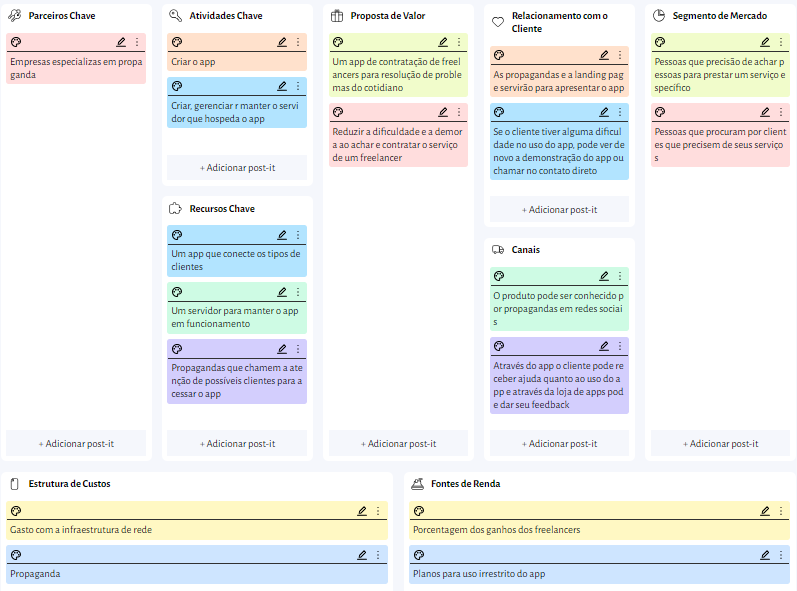
\includegraphics[width=1\textwidth]{fotos/canvas.png}
\SourceOrNote{Autoria própria (2024)}
\end{figure}

    O seu formato de tabela separa por cessão cada ponto importante para um negócio se manter.

\end{document}